% 6-8 pages.
% Due May 31, 2016.

\documentclass[11pt]{article}

\usepackage[T1]{fontenc}
\usepackage{lmodern}
\usepackage{hyperref}
\usepackage[ruled, linesnumbered]{algorithm2e}
\usepackage{bm}
\usepackage{epsf,graphicx,amssymb,amsmath,amsbsy,authblk}
\usepackage[english]{babel}
\usepackage{psfrag}
\usepackage{fancyhdr}
\usepackage{mathrsfs}
\usepackage{natbib}
\usepackage{xcolor}

% Algebraic rings.
\newcommand*{\Complex}{\mathbb{C}}
\newcommand*{\Binary}{\mathbb{F}_2}
\newcommand*{\Ints}{\mathbb{Z}}
\newcommand*{\Reals}{\mathbb{R}}

% Operators.
\renewcommand*{\L}{\mathscr{L}}
\renewcommand*{\O}{\mathcal{O}}
\renewcommand*{\d}[3][1]{%
    \if#11
    \frac{d #2}{d #3}
    \else
    \frac{d^#1 #2}{d #3^#1}
    \fi%
}
\newcommand*{\half}{^{1/2}}
\newcommand*{\invhalf}{^{-1/2}}
\newcommand*{\ip}[2]{\left<#1, #2\right>}
\newcommand*{\p}[3][1]{%
    \if#11
    \frac{\partial #2}{\partial #3}
    \else
    \frac{\partial^#1 #2}{\partial #3^#1}
    \fi%
}

% Matrices.
\newcommand*{\A}{\mathbf{A}}
\renewcommand*{\H}{\mathbf{H}}
\newcommand*{\I}{\mathbf{I}}
\renewcommand*{\P}{\mathbf{P}}
\newcommand*{\X}{\mathbf{X}}
\newcommand*{\W}{\mathbf{W}}
\newcommand*{\PHI}{\mathbf{\Phi}}
\newcommand*{\PSI}{\mathbf{\Psi}}
\newcommand*{\SIGMA}{\mathbf{\Sigma}}

% Vectors.
\renewcommand*{\a}{\mathbf{a}}
\renewcommand*{\c}{\mathbf{c}}
\newcommand*{\f}{\mathbf{f}}
\newcommand*{\ft}{\tilde{\f}}
\renewcommand*{\r}{\mathbf{r}}
\newcommand*{\w}{\mathbf{w}}
\newcommand*{\x}{\mathbf{x}}
\newcommand*{\z}{\mathbf{z}}
\newcommand*{\epsilonv}{\bm{\epsilon}}
\newcommand*{\phiv}{\bm{\phi}}
\newcommand*{\psiv}{\bm{\psi}}
\newcommand*{\zero}{\mathbf{0}}

% hyperref commands.
\renewcommand*{\sectionautorefname}{Section}
\renewcommand*{\subsectionautorefname}{\sectionautorefname}

% Other commands.
\newcommand{\KSE}{Kuramoto--Sivashinsky equation}
\newcommand{\kkc}[1]{\textcolor{red}{[KKC: #1]}}

\marginparwidth 0pt
\oddsidemargin 0pt
\evensidemargin 0pt
\marginparsep 0pt
\topmargin -50pt
\textwidth 17cm
\textheight 22.0cm
\headheight 13.6pt
\pagestyle{fancy}

\lhead{{\it Montestigliano Workshop}}
\rhead{{\it 2016 Reports}}

% Bibliography styles.
\bibliographystyle{plainnat}
\setcitestyle{}

\graphicspath{{figures/}}

\begin{document}

\begin{center}
    {\bf \Large Modeling the Kuramoto--Sivashinsky Equation}\\
    \vspace{0.3cm}
    {%
        \large{%
            Victor Beltran,\footnote{Universidad Polit\'ecnica de Madrid}
            Kevin K. Chen,\footnote{University of Southern California}
            Emma Cooke,\footnote{Imperial College London} and
            Simon Pasche\footnote{\'Ecole Polytechnique F\'ed\'erale de Lausanne}%
        }%
    }
\end{center}
\vspace{0.3cm}

\begin{abstract}
    We investigate the nonlinear dynamics and modeling of the \KSE.
    Both the common parallel equation with periodic boundary conditions, as well as a non-parallel equation on an infinite domain, are considered.
    In both equations, we report three cases where the stable solution is the trivial solution, a simple periodic orbit of a single frequency, and a more complex periodic orbit exhibiting multiple harmonics.
    In particular, the parallel periodic equation has analytical eigenvalues and eigenmodes, which allow an simple characterization of the Hopf bifurcation.
    The various types of solutions are demonstrated with phase portraits.
    Next, we compute POD-DEIM modes and reduced-order models for the parallel equation.
    Not only does POD-DEIM capture the limit cycle with a comparatively small number of modes, but also, transient modes correctly capture the limit cycle, and limit cycle modes correctly capture the transients.
\end{abstract}

\section{Introduction}

The \KSE\ is a fourth-order partial differential equation in time and one-dimensional space that arises in many physical phenomena.
The equation was independently discovered by \cite{KuramotoPTP76} in the context of wave propagation in reaction--diffusion systems, and \cite{SivashinskyAA77} in the context of laminar flames.
Since then, the equation has also been derived for thin film flows, interfacial instabilities, drift waves in plasmas \citep[see][]{KevrekidisSIAMJAM90}, Tollmien--Schlichting waves in flat-plate boundary layers \citep{FabbianeAMR14}, and many more applications.

One of the features that makes the \KSE\ a common model problem is the complex hierarchy of attractors for different equation parameters.
The range of stable solutions, as discussed by \cite{KevrekidisSIAMJAM90}, includes fixed points, simple periodic orbits, more complex periodic orbits (e.g., exhibiting multiple frequencies), quasi-periodic orbits, and ultimately chaos.
Therefore, many have characterized the equation's complex dynamics using simple reduced-order models, often taking advantage of symmetry \citep[e.g.,][]{AubrySIAMJSC93, RowleyPD00}.

Proper orthogonal decomposition---also known as principal component analysis and Karhunen--Lo\`eve expansion---is a very common data-based modal decomposition, and is discussed in works by \cite{SirovichQAM87} and \cite{HolmesTCSDSS}.
Given a set of data snapshots, the technique extracts orthogonal modes that optimally capture the energy of the input data.
These modes are then typically used in Galerkin models to form reduced order models.
Despite the popularity of POD-based reduced order models, the technique suffers from a number of shortcomings.
In particular, the construction of nonlinear terms in POD models may be computationally expensive.

The discrete empirical interpolation method \citep[DEIM;][]{ChaturantabutIEEECDC09, ChaturantabutRice09a} addresses the last concern by intelligently selecting discrete points in the domain for which the nonlinear term is computed, and neglecting all other points.
Although other nonlinear POD models exist \citep[see, e.g.,][]{NoackJFM03}, the DEIM method has been shown to be very computationally efficient and to create very accurate POD models.
Although error bounds have been derived for DEIM, the precise reasons for its success have not been rigorously proven.

In this report, we cover two topics related to the \KSE.
First, we use linear stability theory and computation to characterize the equation's simple attractors.
Second, we demonstrate the success of POD-DEIM reduced-order models for this equation.
The \KSE\ and POD-DEIM are first reviewed in \autoref{sec:theory}.
Next, the attractors are described in \autoref{sec:attractors}, and the application of POD-DEIM is demonstrated in \autoref{sec:pod-deim}.
Finally, we summarize our work in \autoref{sec:conclusions}.

\section{Theory}
\label{sec:theory}

\subsection{The \KSE}
\label{sec:ks}

In this report, we cover two different forms of the \KSE.
Given the streamwise displacement $x$ and time $t$, the dependent variable $w(x, t) : \Reals \times \Reals \to \Reals$ obeys the nonlinear equation
\begin{equation}
    \label{eq:ks}
    \p{w}{t} = \L w - w \p{w}{x},
\end{equation}
where the linear operator $\L$ is given by
\begin{equation}
    \label{eq:ks-linear}
    \L := - \left(U \p{}{x} + \p{}{x} \left(\mu_0 \p{}{x}\right) + \gamma \p[4]{}{x}\right).
\end{equation}

In the parallel form, we assume a periodic domain $x \in [-1, 1]$.
We also define positive real constants $U, \mu_0, \gamma$ respectively corresponding to the advection velocity, anti-diffusion, and short-wavelength diffusion.
The role of each term can be seen by examining a snapshot in time of the form $w = e^{i \pi n x}$ for wavenumbers $n \in \Ints$.
The two first derivative terms correspond to advection at the speed $U + w$, as in the Burgers' and Navier--Stokes equation;
the second derivative term evaluates to $(\pi n)^2 \mu_0 w$ and is therefore antidiffusive and destabilizing;
and the fourth derivative term evaluates to $- (\pi n)^4 \gamma w$ and is therefore diffusive and stabilizing, especially at short wavelengths.
The non-parallel form of the \KSE\ that we will consider is the same, except that we employ $\mu_0(x) = e^{-x^2}$ and consider the infinite domain $x \in \Reals$, where assume that $w$ is well-behaved at $x \to \pm \infty$.

For both forms, we remark that the $U \, \partial / \partial x$ term is actually optional---$w$ could be replaced with $U + w$ and the $U \, \partial / \partial x$ term removed, and the equations will remain the same.
In fact, most works omit the $U \, \partial / \partial x$ term in their analyses.
The purpose of this term is to allow the base flow to be fixed at $w(x, t) = 0$, which corresponds to an advection speed of any arbitrary $U$.

\subsection{POD-DEIM}

Proper orthogonal decomposition \citep{SirovichQAM87, HolmesTCSDSS} is a method of identifying dominant directions in a size $m$ set of data $\{\x_k\}_{k=1}^m$, with $\x_k \in \Complex^n$ for $k = 1, \ldots, m$.
(It is common in many problems to restrict $\x_k$ to $\Reals^n$.)
The modes are ranked in a particular order so the first $r$ modes maximize the orthogonal projection of the data onto the span of those modes for each $r = 1, \ldots, m$.
Given an inner product $\ip{\cdot}{\cdot} : \Complex^n \times \Complex^n \to \Complex$ and the Kronecker delta $\delta_{jk}$, we therefore write the POD modes as the set of vectors $\phiv_j \in \Complex^n$ for $j = 1, \ldots, m$ such that
\begin{subequations}
    \begin{align}
        \sum_{k=1}^m \left\|\x_k - \sum_{j=1}^r \ip{\x_k}{\phiv_j} \phiv_j \right\|_2^2 \quad & \text{is minimized for each } r = 1, \ldots, m, \\
        \ip{\phiv_j}{\phiv_k} = \delta_{jk}.
    \end{align}
\end{subequations}
In reduced-order modeling, it is common to truncate the POD mode set and only consider the proper subset $\{\phiv_j\}_{j=1}^r$ for $1 \le r \ll m$, with the assumption that most interesting features of $\{\x_k\}_{k=1}^m$ are contained in only $r$ modes.

The computation of POD is straightforward.
Let us assume the common case where $m \le n$, and let $(\cdot)^*$ indicate the conjugate transpose.
Also, consider the inner product $\ip{\cdot}{\cdot} : \Complex^n \times \Complex^n \to \Complex; \z_j, \z_k \mapsto \z_k^* \H \z_j$, where typically, $\H \in \Reals^{n \times n}$ is a diagonal matrix with the positive grid sizes on the diagonal.
(On uniform grids, we would normally have $\H = \I$.)
Given the data matrix $\X := \begin{bmatrix} \x_1 & \ldots & \x_m \end{bmatrix} \in \Complex^{n \times m}$, the economy-sized singular value decomposition (SVD) of $\H\half \X$ is
\begin{equation}
    \label{eq:svd}
    \H\half \X = (\H\half\PHI) \SIGMA \W^*,
\end{equation}
where $\PHI \in \Complex^{n \times m}$ and $\PHI^* \H \PHI = \I$, $\SIGMA \in \Reals^{m \times m}$ is a diagonal matrix with $\{\sigma_k\}_{k=1}^m$ on the diagonal such that $\sigma_1 \ge \cdots \ge \sigma_m \ge 0$, and $\W \in \Complex^{m \times m}$ and $\W^* \W = \W \W^* = \I$.
The POD modes are then the columns of $\PHI = \begin{bmatrix} \phiv_1 & \cdots & \phiv_m \end{bmatrix}$.

The primary challenge in nonlinear modeling is to capture nonlinear dynamics in a way that is both accurate and computationally efficient.
The POD-DEIM algorithm \citep{ChaturantabutIEEECDC09, ChaturantabutRice09a} addresses this issue as follows.
Suppose that the discrete-space dynamics contain the nonlinear function $\f : \Complex^n \to \Complex^n$, and the dynamics are given for $\x(t) : \Reals \to \Complex^n$ by
\begin{equation}
    \d{\x}{t} = \A \x + \f(\x).
\end{equation}
We restrict $\x$ to the span of $\{\phiv_j\}_{j=1}^r$ by assigning POD mode coefficients $\a(t) := \begin{bmatrix} a_1(t) & \cdots & a_r(t) \end{bmatrix} : \Reals \to \Complex^r$ such that $\x(t) = \PHI \a(t)$.
Using this projection, we arrive at
\begin{equation}
    \label{eq:galerkin}
    \d{\a}{t} = \PHI^* \H \A \PHI \a + \PHI^* \H \f(\PHI \a),
\end{equation}
but the nonlinear term must still be computed over $\Complex^n$.

Therefore, we also compute POD modes $\psiv_j \in \Complex^n$ for $j = 1, \ldots, s$ from the nonlinear terms $\f(\x_1), \ldots, \f(\x_m)$, and we define $\PSI := \begin{bmatrix} \psiv_1 & \cdots & \psiv_s \end{bmatrix}$.
Next, we project the output of $\f$ to the span of $\{\psiv_j\}_{j=1}^s$, such that for some coefficient vector $\c \in \Complex^s$, error vector $\epsilonv \in \Complex^n$, and input $\x \in \Complex^n$,
\begin{equation}
    \f(\x) = \PSI \c + \epsilonv
\end{equation}
and $\ip{\epsilonv}{\psiv_j} = 0$ for $j = 1, \ldots, s$.
To reduce the computation of $\f$ to one over $\Complex^s$, we use the DEIM algorithm (Algorithm~\ref{algo:deim})%
\begin{algorithm}[t]
    \caption{
        Discrete empirical interpolation method;
        $\PSI_j$ and $\P_j$ respectively denote the matrices comprised of first $j$ columns of $\PSI$ and $\P$, and $P_{j, k}$ denotes the entry of $\P$ in row $j$ and column $k$.%
    }
    \label{algo:deim}

    \DontPrintSemicolon
    \SetAlgoLined

    \KwData{Nonlinear POD modes $\PSI := \begin{bmatrix} \psiv_1 & \cdots & \psiv_s \end{bmatrix} \in \Complex^{n \times s}$}
    \KwResult{DEIM projection matrix $\P \in \Binary^{n \times s}$}

    $m \leftarrow \arg \max |\psiv_1|$ \;
    $\P \leftarrow 0^{n \times s}$ \;
    $P_{m, 1} \leftarrow 1$ \;
    \For{$j = 2, \ldots, s$} {
        $\r \leftarrow (\I - \PSI_{j-1} (\P_{j-1}^* \PSI_{j-1})^{-1} \P_{j-1}^*) \psiv_j$ \;
        $m \leftarrow \arg \max |\r|$ \;
        $P_{m, j} \leftarrow 1$ \;
    }
\end{algorithm}
to choose a projection matrix $\P \in \Binary^{n \times s}$ that consists of all zeros, except that each column has one unique index for which the entry is one.
Thus, $\P^* \f(\x) = \P^* \PSI \c + \P^* \epsilonv$; if $\P^* \PSI$ is full-rank, then $\c = (\P^* \PSI)^{-1} \P^* (\f(\x) - \epsilonv)$, and hence,
\begin{equation}
    \label{eq:nonlinear-projection}
    \f(\x) = \PSI (\P^* \PSI)^{-1} \P^* \f(\x) + (\I - \PSI (\P^* \PSI)^{-1} \P^*) \epsilonv.
\end{equation}

To complete the POD-DEIM procedure, we make two assumptions: first, we assume that
\begin{equation}
    \label{eq:zero-error}
    (\I - \PSI (\P^* \PSI)^{-1} \P^*) \epsilonv = \zero
\end{equation}
(i.e., the nonlinear POD modes perfectly capture the nonlinear dynamics), and second, we assume that there exists a pointwise version $\ft : \Complex^s \to \Complex^s$ of $\f$ such that
\begin{equation}
    \label{eq:pointwise}
    \P^* \f(\x) = \ft(\P^* \x).
\end{equation}
That is, $\P^* \f(\x)$ first computes $\f(\x)$ and then selects discrete elements of the output to keep; on the other hand, $\ft(\P^* \x)$ first selects discrete elements of the \emph{input}, and computes the nonlinearity only on those elements.
We remark that this shortcut is generally allowed, even if $\f$ does not appear to be a pointwise operation, e.g., if it involves spatial derivatives.
For instance, suppose that $\f(\x)$ is the discrete-space formulation of the function $f(w) = -w \, \partial w / \partial x$, as in~\eqref{eq:ks}.
To evaluate $\ft(\P^* \x)$, one would simply evaluate both $-w$ and $\partial w / \partial x$ at the DEIM points $x_j$ corresponding to the nonzero elements of the columns of $\P$, and multiply the result.

Finally, we combine (\ref{eq:galerkin}, \ref{eq:nonlinear-projection}, \ref{eq:zero-error}, \ref{eq:pointwise}) to obtain the reduced-order model
\begin{equation}
    \d{\a}{t} = \PHI^* \H \A \PHI \a + \PHI^* \H \PSI (\P^* \PSI)^{-1} \ft(\P^* \PHI \a).
\end{equation}
The matrices $\PHI^* \H \PSI (\P^* \PSI)^{-1} \in \Complex^{r \times s}$ and $\P^* \PHI \in \Complex^{s \times r}$ should be pre-computed for maximal efficiency.
We remark that it is never actually necessary to represent or use $\P^*$ explicitly in computations; in software, it is sufficient just to use its nonzero entries to manipulate the indices of its operand.
In addition, we will employ $s = r$ for simplicity in this report.

\section{Numerical methods}
\label{sec:methods}

In the parallel \KSE, we use the Fourier pseudospectral method described by \cite{WeidemanACMTMS00} to compute differentiation matrices.
To reduce minimize the amplification of short-wavelength noise by the fourth derivative, we employ the 36th order filter described by \cite{HouJCP07} for the diffusion term.
We use the uniform spatial discretization $\Delta x = 0.005$, such that the periodic domain $x \in [-1, 1]$ is comprised of 400 grid points.
The parallel equation is simulated and analyzed in MATLAB.

In the non-parallel \KSE, we use the finite element software FreeFem++ \citep{HechtJNM12}, employing 4,000 equispaced elements with width $\Delta x = 0.05$ on the domain $x \in [-100, 100]$.
Homogeneous Dirichlet conditions are set at $x = -100$, and outflow conditions are set at $x = 100$.
The shift-and-invert variant of the Arnoldi method \citep[see][]{TrefethenNLA} is used to compute the leading eigenvalues and eigenmodes of the linearized dynamics.

\section{Characterizations of attractors}
\label{sec:attractors}

\subsection{Parallel equation}

In the parallel equation, the eigendecomposition of the linear dynamics $\L$ about the base flow $w(x) = 0$ can be expressed analytically.
Because of the domain periodicity, we assume eigenmodes of the form $w_n(x) = e^{i \pi n x}$ for $n \in \Ints$.
The eigendecomposition $\L w_n = \lambda_n w_n$, for $\lambda_n \in \Complex$, therefore yields $\lambda_n = (\pi n)^2 (\mu_0 - (\pi n)^2 \gamma) - i \pi n U$.
Then $n = 0$ eigenmode---corresponding to $\lambda_0 = 0$---is simply the mode where $w(x)$ is a constant, and is related to the arbitrary velocity scale discussed in \autoref{sec:ks}.
Besides this mode, all other eigenmodes have a nonzero imaginary part.
Examining the structure of the real part of $\lambda_n$, it is evident that the $n = \pm 1$ mode is the least stable mode.
In particular, the $n = \pm 1$ mode undergoes a Hopf bifurcation when $\gamma = \mu_0 / \pi^2$.
The corresponding eigenvalue reveals that the base flow is stable when $\gamma > \mu / \pi^2$ and unstable when $\gamma < \mu / \pi^2$.

\kkc{Fill in the rest.}

\autoref{fig:time-resolved}(a) depicts\ldots

\begin{figure}
    \centering
    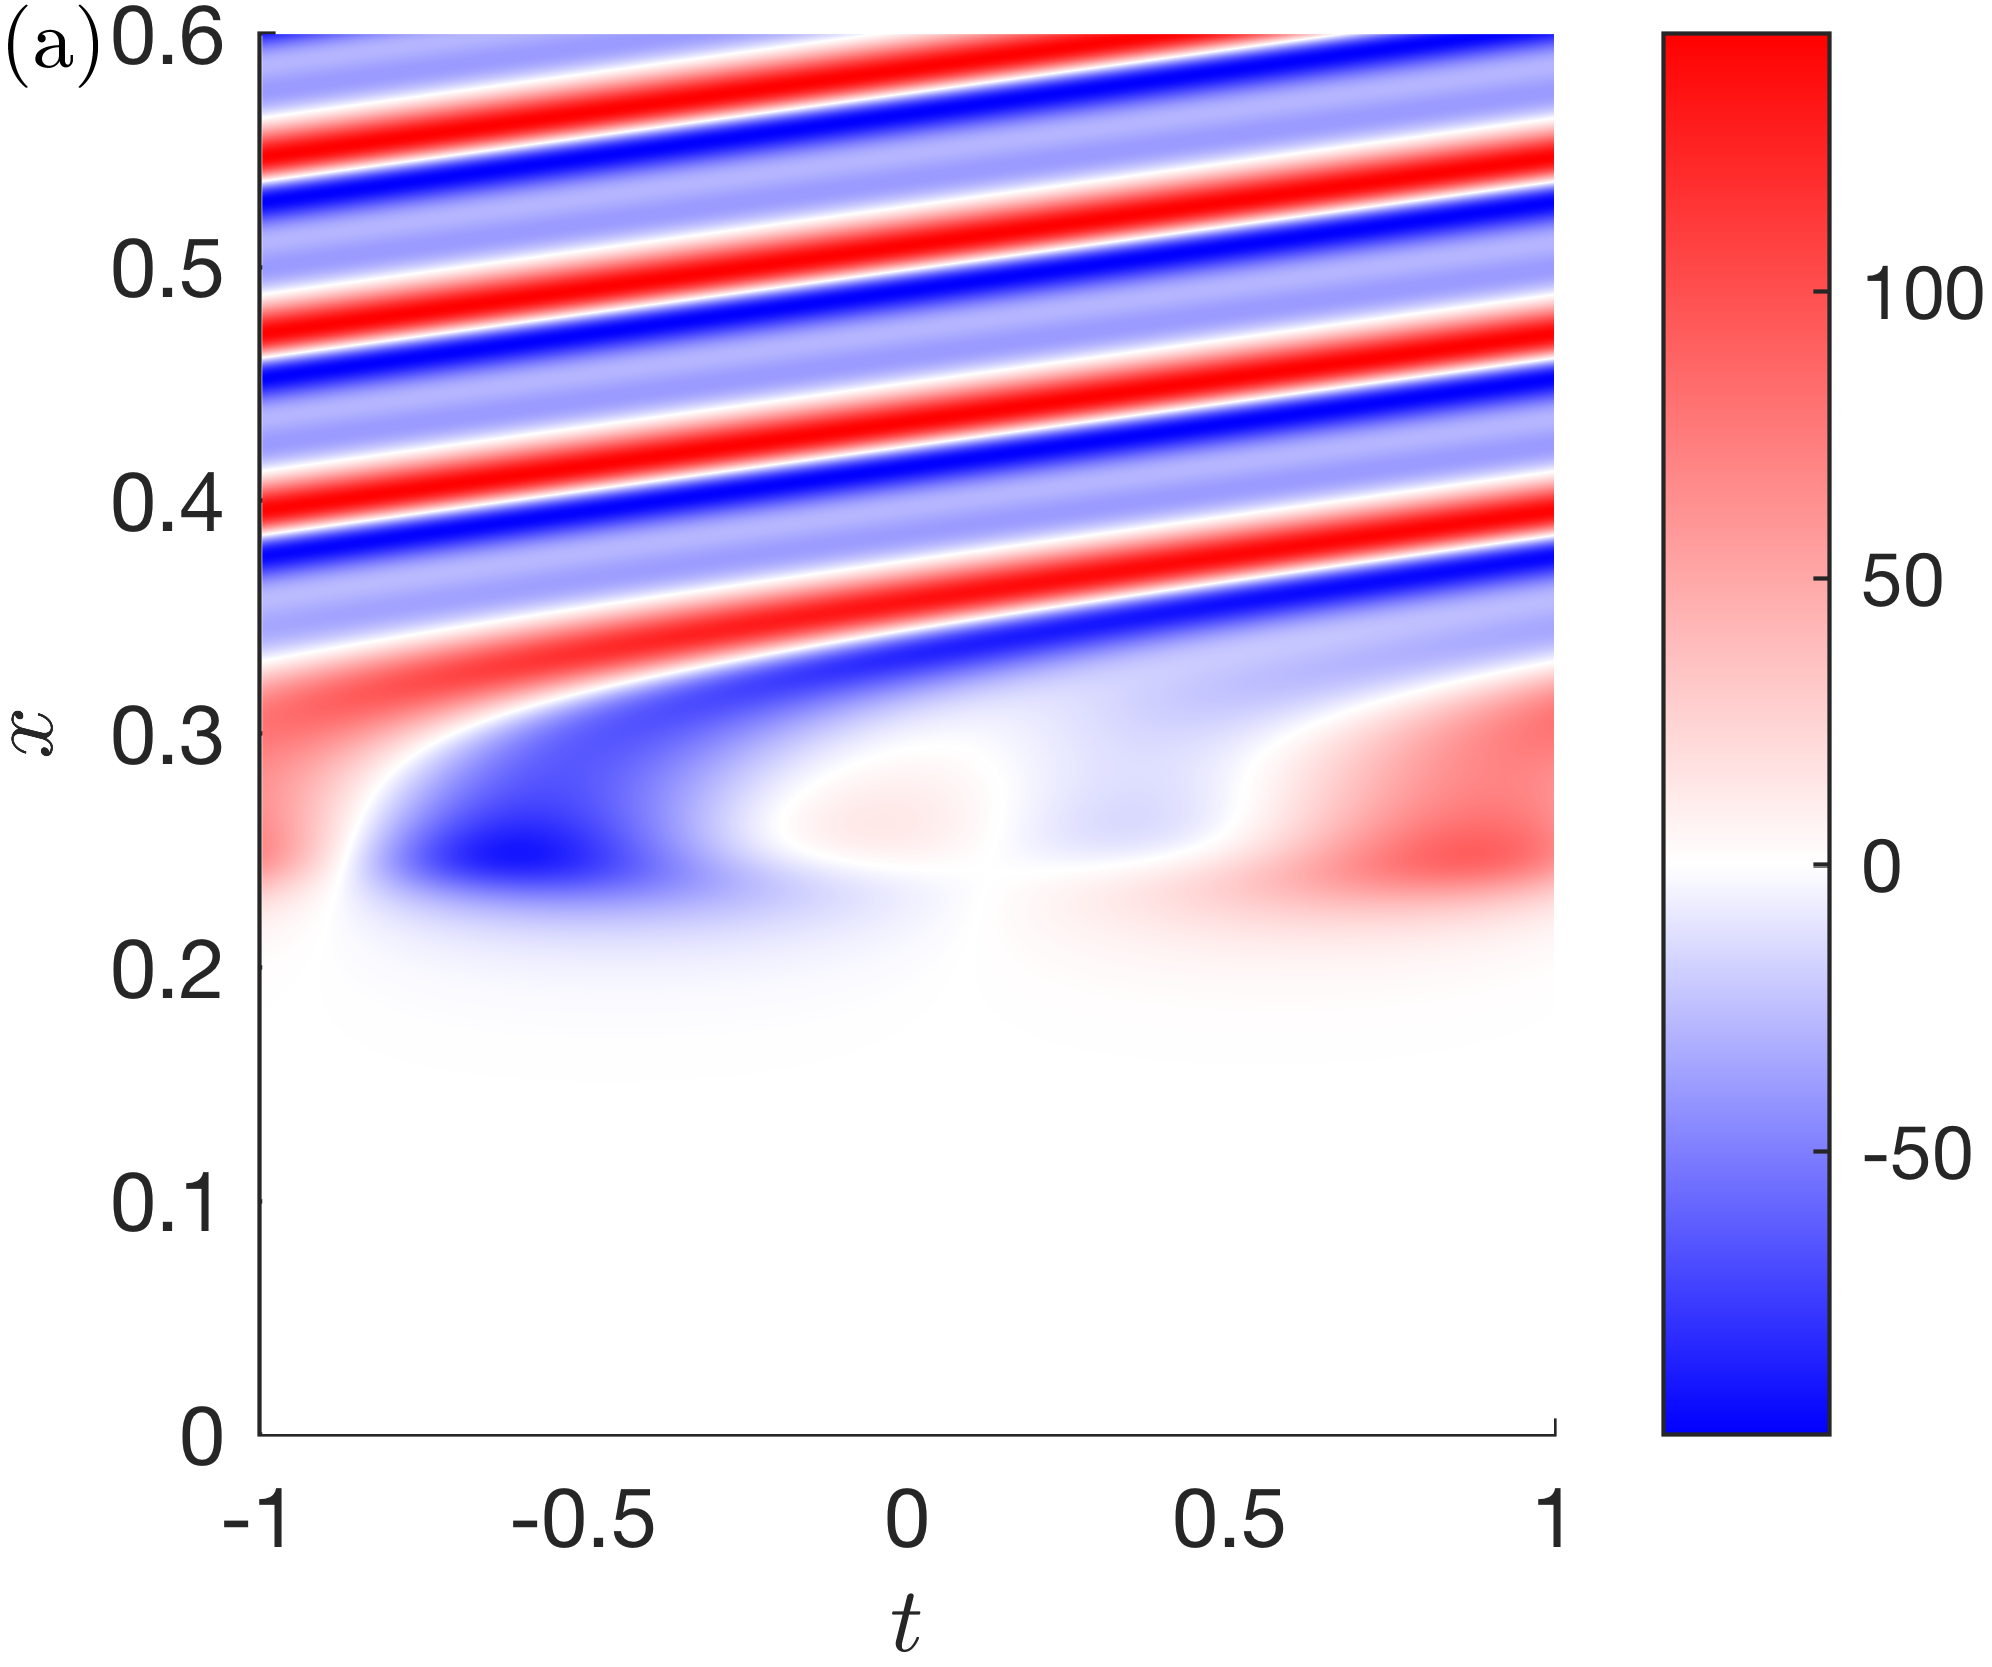
\includegraphics{xt_parallel}
    \hfill
    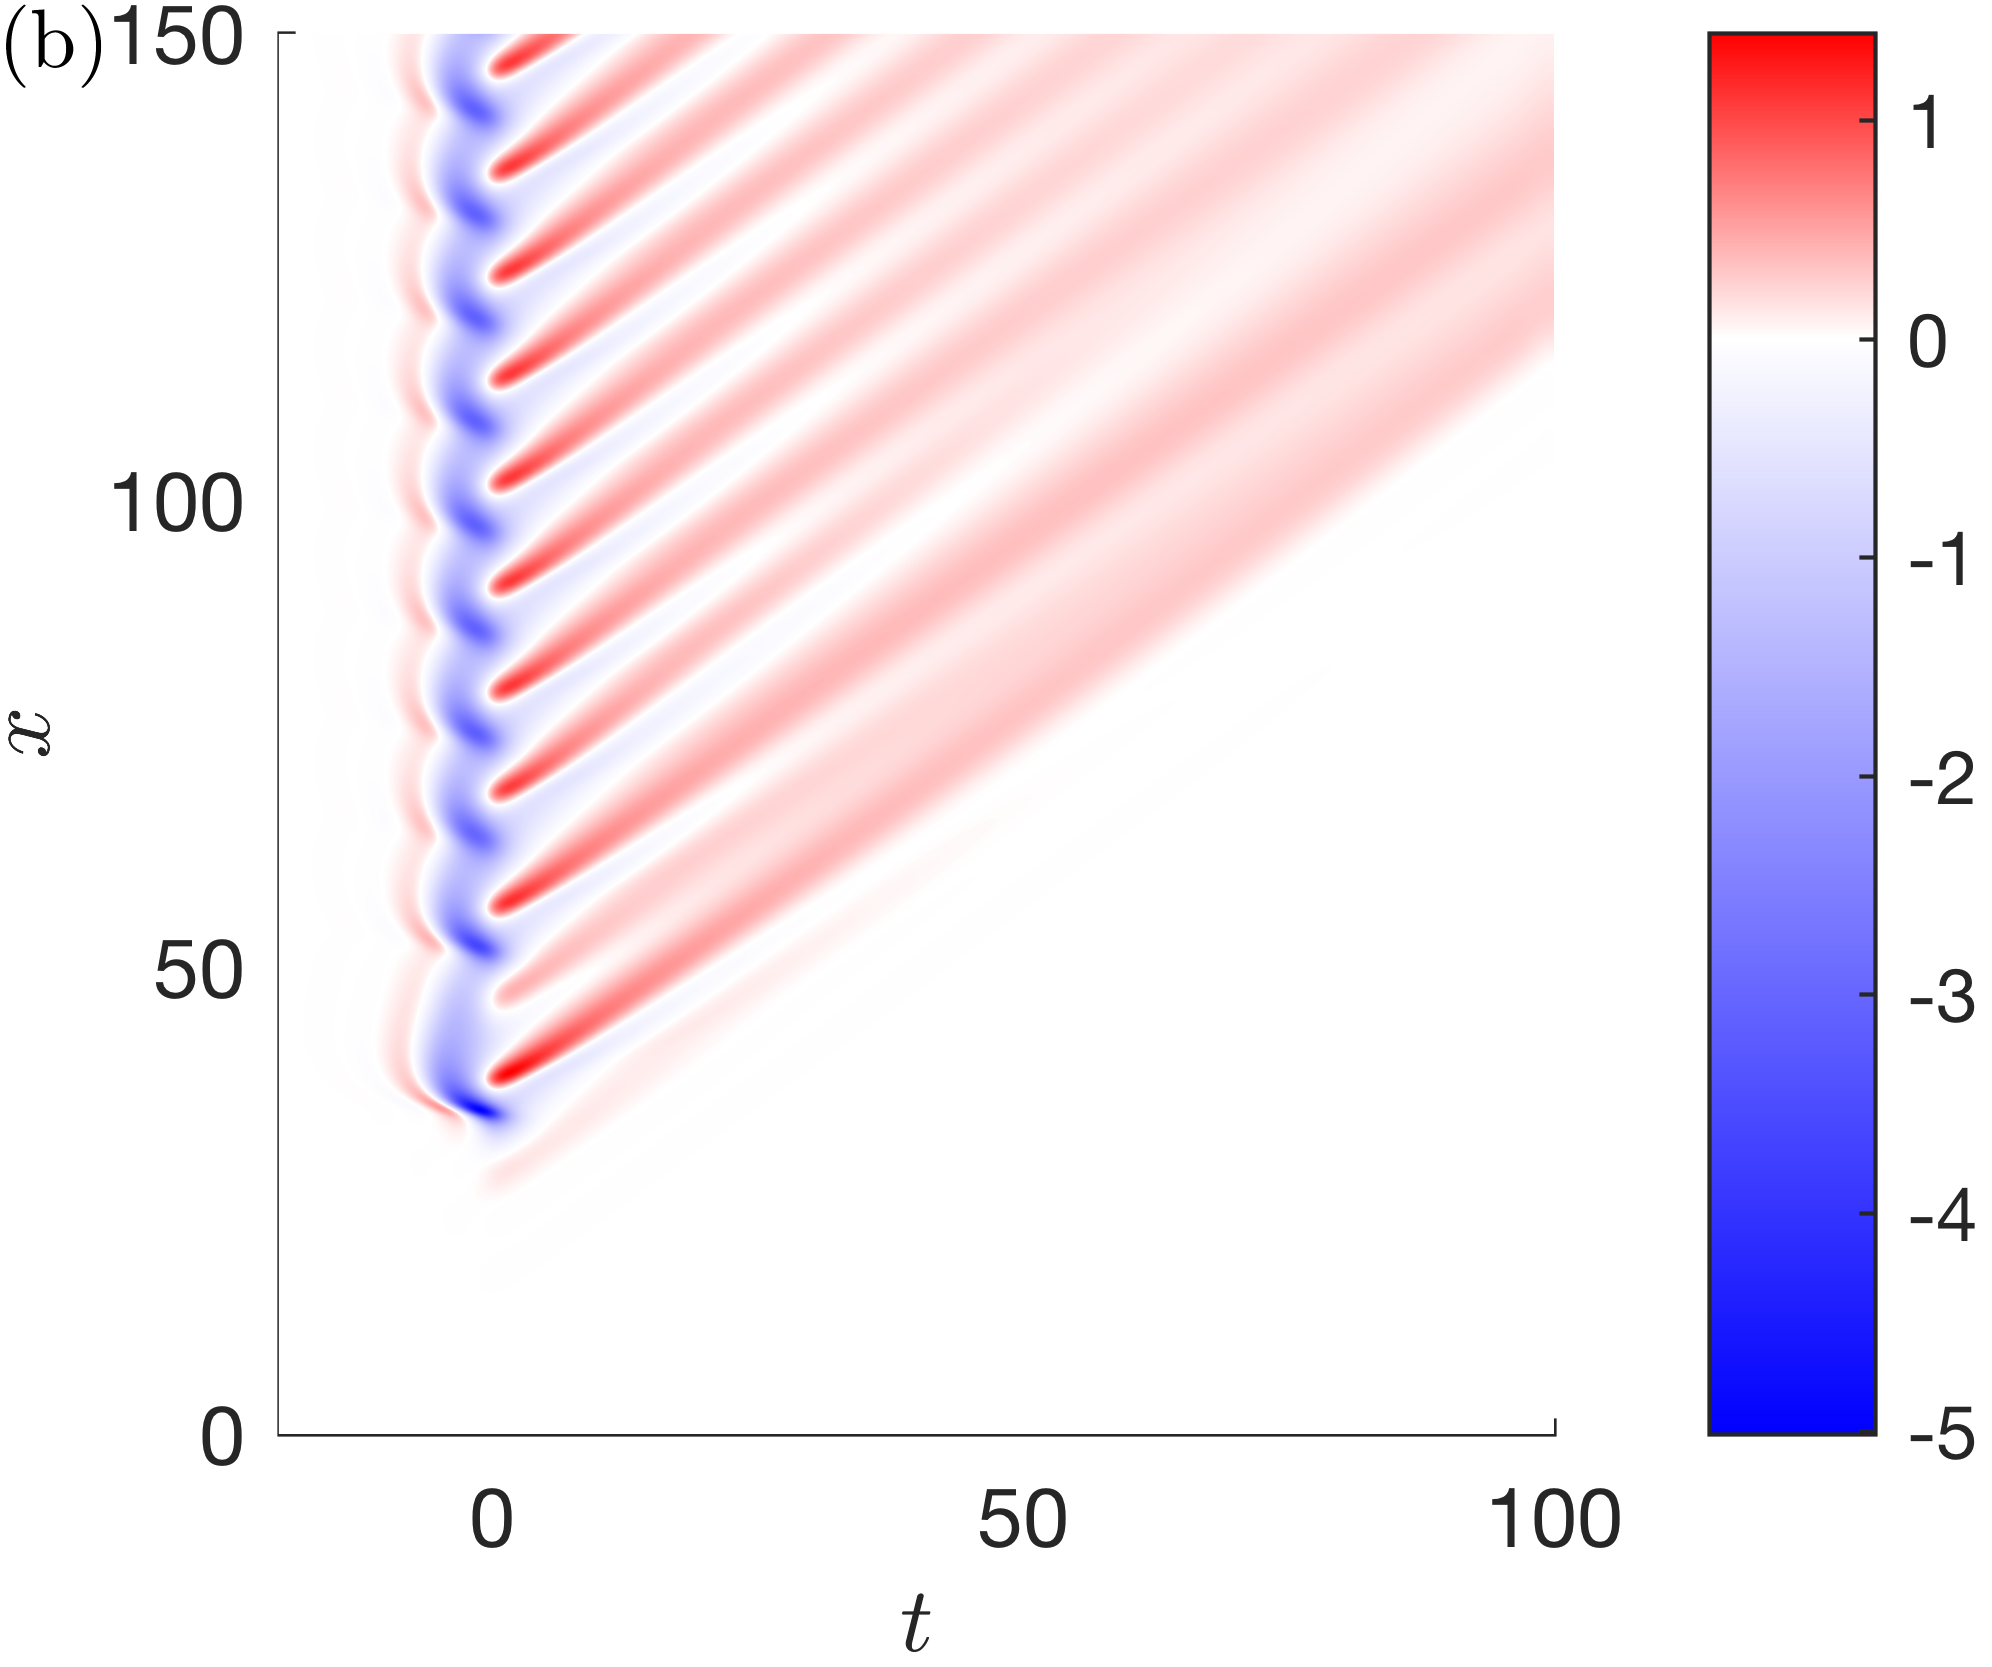
\includegraphics{xt_nonparallel}

    \caption{%
        $x$--$t$ plots of the \KSE, starting from a small random initial condition.
        (a) The parallel equation, with $\mu_0 = \pi^2$ and $\gamma = 0.28$.
        (b) The nonparallel equation, with $\mu_0 = 3.95$ and $\gamma = 1$.%
    }
    \label{fig:time-resolved}
\end{figure}

\subsection{Non-parallel equation}

\autoref{fig:time-resolved}(b) depicts\ldots

\section{POD-DEIM models of the parallel equation}
\label{sec:pod-deim}

\section{Conclusions}
\label{sec:conclusions}

We have analyzed the parallel and non-parallel {\KSE}s from the perspective of stable solutions and POD-DEIM models.
The eigendecomposition of the linearized parallel dynamics about the trivial base flow reveals that the longest wave mode is the least stable one.
On the other hand, the eigendecomposition of the non-parallel equation is treated numerically.
When the coefficient of the stabilizing fourth derivative is decreased, the stable solution of both equations evolves from the base flow to a simple periodic orbit of a single frequency, and further to a periodic orbit exhibiting multiple harmonics.

In the parallel equation, the state POD modes are simple sinusoids.
The DEIM points are scattered throughout the domain because the periodicity creates spatial invariance.
Considering only the saturated periodic orbit, 8-mode POD-DEIM models capture simple periodic orbits extremely well, and 6-mode models exhibit small errors the time periodicity.
Furthermore, POD-DEIM models computed only from the transient growth, as well as only from the periodic orbit, are both able to capture the entirety of the transient and saturated dynamics.
A greater number of modes may be required for accurate modeling, however, especially when the periodic orbit exhibits multiple frequencies.

\section{Acknowledgements}

We would like to thank ERCOFTAC for funding and providing the 2016 Montestigliano Spring School.
We are also deeply grateful for Denis Sipp, Peter Schmid, and Shervin Bagheri for leading the school.
K. K. C. was supported by the Viterbi Postdoctoral Fellowship through the Viterbi School of Engineering at the University of Southern California.
\kkc{Victor, Emma, Simon---add your funding sources and other acknowledgements here.}

\bibliography{BeltranChenCookePasche}

\end{document}

%%% Local Variables:
%%% mode: latex
%%% TeX-master: t
%%% End:
